\documentclass[12pt]{article}
%encoding
%--------------------------------------
\usepackage[utf8]{inputenc}
\usepackage[T1]{fontenc}
\usepackage{listings}
\usepackage{minted}
\usepackage{mathtools}
\usepackage{graphicx}
\usepackage{placeins}  

\graphicspath{ {./img/} }

%--------------------------------------

%German-specific commands
%--------------------------------------
\usepackage[ngerman]{babel}
%--------------------------------------

%Hyphenation rules
%--------------------------------------
\usepackage{hyphenat}
\hyphenation{Mathe-matik wieder-gewinnen}
\usepackage{lipsum}
%--------------------------------------
\begin{document}
\pagenumbering{gobble}
\clearpage
\thispagestyle{empty}
\author{Rafael Schreiber}
\date{Januar 2021}
\title{Berechnung der Kreiszahl $\pi$ mithilfe der Leibniz' Formel}
\maketitle
\clearpage
\pagenumbering{arabic}
\tableofcontents
\newpage

\section{Einleitung}
\subsection{Aufgabenstellung}
Laut der Angabe ist das Ziel dieses Programms die Kreiszahl $\pi$ zu berechnen. 
Dabei soll die Leibniz' Formel \cite{leibnizformular} zur Annäherung an die 
Zahl verwendet werden.
\begin{center}
$\sum_{k=0}^{\infty}{\frac{(-1)^{k}}{2k+1}}=1-{\frac{1}{3}}+
{\frac{1}{5}}-{\frac{1}{7}}+{\frac{1}{9}}-\dotsb={\frac{\pi}{4}}$
\end{center}
Wie in der Formel zu erkennen ist, gibt es positive und negative Terme. 
In der geforderten Implementierung wird erwartet, dass die negativen und 
positiven Terme auf je zwei Prozesse aufgeteilt werden, damit die jeweiligen 
Ergebnisse parallel und damit auch hoffentlich  schneller berechnet werden 
können.
\newline
Die Angabe schreibt vor, dass der Elternprozess diese zwei Kindprozesse 
erstellt und dann darauf wartet, bis die Kindprozesse ihre Terme fertig 
berechnet haben. Die jeweils positiven und negativen Ergebnisse werden in 
eine Textdatei geschrieben, welche dann vom Elternprozess ausgelesen wird, 
damit dieser die entgültige Berechnung durchführen kann.
\newpage
\begin{figure}[htbp]
    \centering
    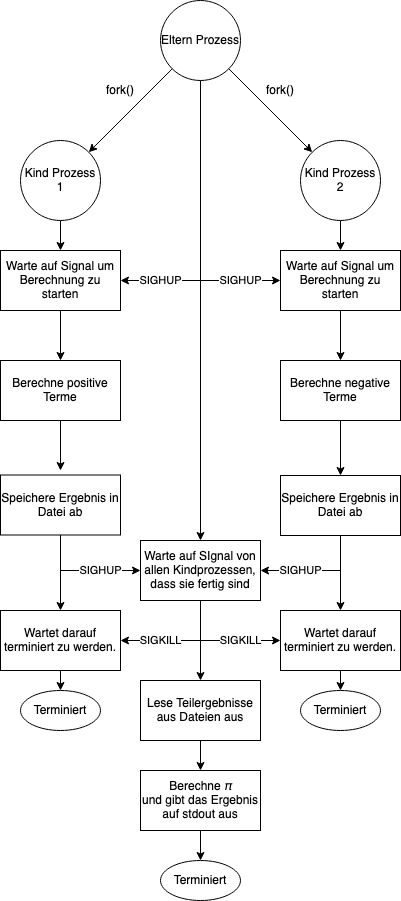
\includegraphics[scale=0.57]{execution_diagram}
    \caption{Ablaufdiagramm des picalc Programms}
    \label{fig:situation1}
\end{figure}
\FloatBarrier
\newpage
\section{Implementierung}
Zu aller erst wurden sämtliche Codierungsrichtlinien von Professor Dr. Günter 
Kolousek eingehalten. Für die Benennung von Variablen und Funktionen wurde 
"\texttt{sneak\_case}" verwendet. Für eine einfachere Kodierung wurden außerdem 
mehrere externe Bibliotheken verwendet, auf welche im Abschnitt 2.2 näher 
eingegangen werden.
\subsection{Erklärung bestimmter Codeteile}
\subsubsection{Nutzung von \texttt{\_\_float128} für mehr Präzision}
Bei der Berechnung von irrationalen Zahlen wie $\pi$ oder e ist das Ziel, auf
soviele Nachkommastellen wie nur möglich zu kommen. Die Anzahl der
Nachkommastellen wird als Präzision bezeichnet. Diese muss auch hoch sein,
um das Ergebnis auf soviele Nachkommastellen wie nur möglich berechnen
und darstellen zu können.
\newline
\texttt{\_\_float128} ist der zugehörige Datentyp für das "`Quadruple-precision 
floating-point format"'  welches in der aktuellen Fassung des IEEE 754-2008
\cite{ieee754} Standards beschrieben ist.
\newline
Das Problem dabei ist, dass nicht jeder Compiler bzw. jedes System diesen
Datentyp unterstützt, deswegen schaut der Präprozessor nach, ob dieser Datentyp
unterstützt wird. Wenn dies nicht der Fall ist, dann wird \texttt{long double} 
zur Speicherung von Kommazahlen verwendet.
\begin{minted}{c++} 
    #ifdef USE_FLOAT128
        typedef __float128  long_double_t;
    #else
        typedef long double long_double_t;
    #endif
\end{minted}
\subsubsection{Umwandlung von \texttt{long\_double\_t} zu \texttt{std::string}}
Ein weiteres Problem ist, wie \texttt{long\_double\_t} zu einem String
konvertiert werden soll. String wird benötigt, weil jeweils die Funktion zum
Speichern der Teilergebnisse sowie die Ausgabe, ein Objekt mit dem Typen 
\texttt{std::string} benötigt. 
\newline
An und für sich existiert die Funktion 
\texttt{std::to\_string()} aber hier ist wieder das Problem mit der Präzision.
Deswegen wurde die Funktion \newline\texttt{to\_string\_w\_precision()}
geschrieben, um dieses Problem zu beheben.
\begin{minted}{c++} 
    template <typename T>
    string to_string_w_precision(const T a_value, const int n = 256){
        ostringstream out;
        out.precision(n);
        out << fixed << a_value;
        string flt = out.str();
        reverse(flt.begin(), flt.end());
        uint8_t trailing_zeros = 0;
        for (char chr : flt){
            if (chr != '0'){
                break;
            }
            trailing_zeros++;
        }
        flt = flt.substr(trailing_zeros, flt.size());
        reverse(flt.begin(), flt.end());
        return flt;
    }
\end{minted}
Diese Funktion erstellt Anfangs einen Puffer, wo die Kommazahl mit einer
beliebigen Präzision \texttt{n} hineingeschrieben werden kann.
Es werden standardmäßig 256 Nachkommastellen verwendet, weil in der Praxis 
diese Genauigkeit sowieso nicht überschritten wird. Da bei Zahlen mit einer
geringeren Präzision die restlichen Nachkommastellen nicht verwendet werden,
sondern mit 0en aufgefüllt werden, werden diese danach aus rein kosmetischen 
Gründen entfernt.
\subsubsection{Algorithmus zur Berechnung der Teilergebnisse}
Das sogennante "`'Herzstück"' dieses Programms ist der Algorithmus zur
Berechnung der Teilergebnisse.
\newpage
\begin{minted}{c++}
    long_double_t calc_part_leibniz(uint64_t n, bool is_positive){ 
        uint8_t startpoint{1};
        if (!is_positive){
            startpoint = 3;
        }
        long_double_t part_result = 0.0;
        for (uint64_t i{0}; i < n; i++){
            part_result += (long_double_t) 1 / (startpoint + 4 * i);
        } 

        if (!is_positive){
            part_result = -part_result;
        }

        return part_result;
    }
\end{minted}
Wie man sehen kann, verlangt diese Funktion zwei Argumente:
\begin{itemize}
    \item \texttt{int n} Anzahl der Schleifendurchläufe, also wie oft der 
    Algorithmus wiederholt wird und somit, wie genau die Annäherung an $\pi$ 
    ist.
    \item \texttt{bool is\_positive} bestimmt ob von der Funktion entweder
    die positiven oder die negativen Terme berechnet werden sollen.
\end{itemize}
Die einzigen Unterschiede zwischen der Berechnung der positiven und der 
negativen Teilergebnisse sind, dass der Startwert im Nenner anders ist
und dass das Ergebnis beim negativen Teilergebnis negiert wird.
\subsubsection{Finale Berechnung der Kreiszahl $\pi$}
Der Teil wofür dieses Programm überhaupt geschrieben wurde befindet sich in
der folgenden Funktion:
\newpage
\begin{minted}{c++}
    void calc_pi(){
        long_double_t pos, neg, pi;
        string pos_str, neg_str;
        string storepath_pos{result_file_path + "part_pos_" + 
                             to_string(getpid()) + ".txt"};
        string storepath_neg{result_file_path + "part_neg_" + 
                             to_string(getpid()) + ".txt"};
        pos_str = tfile::read(storepath_pos.c_str());
        neg_str = tfile::read(storepath_neg.c_str());
        pos = stold(pos_str);
        neg = stold(neg_str);
        pi = (pos + neg) * 4;
        console->info("Final calculation finished. pi = \e[1m{}\e[0m", 
                      to_string_w_precision(pi));
    }
\end{minted}
In dieser Funktion werden zuerst die Dateipfade beider Textdateien 
"`zusammengebaut"' um diese dann mithilfe der Funktion 
\texttt{tfile::read()}, bereitgestellt von der Bibliothek tfile [2.2.3], 
auszulesen. Diese zwei Textdateien enthalten jeweils die positiven und 
negativen Teilergebnisse. Diese Teilergebnisse werden dann mit der Funktion 
\texttt{std::stold()} in den \texttt{long\_double\_t} Datentyp konvertiert, um 
damit rechnen zu können. Das finale Ergebnis, nämlich $\pi$, wird berechnet,
indem das positive und das negative Teilergebnis addiert wird und dieses dann 
mit 4 multipliziert wird. Zuletzt wird das Endergebnis schön formatiert auf 
stdout ausgegeben.
\subsection{Externe Bibliotheken im Einsatz}
Um nicht jede Kleinigkeit selbst programmieren zu müssen und auch weil es von
der Angabe so gefordert wurde, kamen in diesem Programm folgende Bibliotheken 
zum Einsatz.
\subsubsection{CLI11}
CLI11 \cite{cli11} ermöglicht die Erstellung einer schönen 
Komandozeilenschnittstelle mit wenig Programmieraufwand. Diese Bibliothek ist 
eine header-only Bibliothek und bietet auch andere Vorteile wie z.B. eingebaute 
Methoden zum überprüfen von angegebenen Kommandozeilenparametern.
\subsubsection{spdlog}
spdlog \cite{spdlog} ist ebenfalls eine header-only Bibliothek um ein einfaches 
Loggen zu ermöglichen. Das Objekt zum loggen wird in diesem Programm global 
deklariert, damit jede Funktion darüber ihren Output geben kann.
\subsubsection{tfile}
Die ebenfalls header-only Bibliothek tfile \cite{tfile} ist mit ihren 598 LOC 
die kleinste verwendete Bibliothek im ganzen Projekt. Obwohl tfile nicht groß 
ist, bietet sie viele nützliche Funktionen, um den Umgang mit Dateien zu vereinfachen.
\section{Verwendung}
\subsection{Kompilierung}
Die Abhängigkeiten vom Projekt sind:
\begin{itemize}
    \item The Meson Build System \cite{meson}
    \item Die Bibliotheken aufgeführt im Punkt [2.2]
    \item Einen C++ Compiler
\end{itemize}
Getestet wurde die Kompilierung auf folgenden Plattformen:
\begin{itemize}
    \item macOS Big Sur (Apple clang version 12.0.0)
    \item Ubuntu 20.04 LTS (gcc version 9.3.0)
\end{itemize}
Beide Plattformen basieren auf einen Prozessor mit x86 Befehlssatz.
\newline
\newline
Zum kompilieren wechselt man als erstes in das \texttt{build/} Verzeichnis,
welches anfangs leer sein sollte. Zweitens werden mit \texttt{meson ..} die 
build-files generiert und zuletzt wird mit dem Befehl \texttt{ninja} das 
Programm kompiliert. Im selben Verzeichnis sollte dann die Binary
\texttt{picalc} zu finden sein.
\newpage
\subsection{Kommandozeilenparamter}
\subsubsection{-i, --iterations UINT:POSITIVE REQUIRED}
Nach diesem Parameter, wird als Argument die Anzahl der Durchläufe angegeben.
Dabei ist es wichtig darauf zu achten, dass die Anzahl größer gleich 2 sein 
muss. Ist dies nicht der Fall oder wird dieser Parameter garnicht mitgegeben, 
dann weigert das Programm sich zu starten.
\subsubsection{-l, --location TEXT:DIR OPTIONAL}
Mit diesem Parameter kann spezifiziert werden, wo die Textdateien mit den
Teilergebnissen gespeichert werden sollen. Standardmäßig werden diese unter
\texttt{/tmp} abgespeichert. Wenn dies nicht erwünscht ist, dann kann als
Argument ein anderer Speicherort angegeben werden.
\subsubsection{-d, --delete}
Dieser Flag gibt an ob die Dateien mit den Teilergebnissen nach der Berechnung
gelöscht werden sollen. Standardmäßig ist das nicht der Fall, aber wenn man
nicht möchte, dass das System mit Dateien zugemüllt wird, dann macht dieser 
Flag durchaus Sinn.

\begin{thebibliography}{5}
\bibitem{leibnizformular} 
Wikipedia: Leibniz-Reihe
\\\textit{https://de.wikipedia.org/wiki/Leibniz-Reihe}

\bibitem{ieee754} 
754-2019 - IEEE Standard for Floating-Point Arithmetic
\\\textit{https://ieeexplore.ieee.org/document/8766229}

\bibitem{cli11} 
GitHub: CLIUtils/CLI11 command line parser
\\\texttt{https://github.com/CLIUtils/CLI11}

\bibitem{spdlog} 
GitHub:  gabime/spdlog Fast C++ logging library. 
\\\texttt{https://github.com/gabime/spdlog}

\bibitem{tfile} 
GitHub: rec/tfile tiny C++11 file utilities by Tom Ritchford
\\\texttt{https://github.com/rec/tfile}

\bibitem{meson} 
The Meson Build System: Project Website
\\\texttt{https://mesonbuild.com/}

\end{thebibliography}

\end{document}